\documentclass[]{usiinfbachelorproject}
\usepackage{subfig}
\usepackage{caption}
%\usepackage{subcaption}
\usepackage{float}
\usepackage{listings}
\usepackage{graphicx}
\captionsetup{labelfont={bf}}

%\newcommand\subsubsection{\@startsection{subsubsection}{3}{\z@}%
%                {-3.25ex\@plus -1ex \@minus -.2ex}%
%                {1.5ex \@plus .2ex}%
%                {\normalfont\normalsize\bfseries}}
%\newcommand\paragraph{\@startsection{paragraph}{4}{\z@}%
%                {3.25ex \@plus1ex \@minus.2ex}%
%                {-1em}%
%                {\normalfont\normalsize\bfseries}}
\author{Francesco Saverio Zuppichini}

\title{Design Interactive Display Applications}
\subtitle{for Active and Walk-by Contact Personalization}
\versiondate{\today}
\begin{committee}
%With more than 1 advisor an error is raised...: only 1 advisor is allowed!
\advisor[Universit\`a della Svizzera Italiana, Switzerland]{Prof.}{Marc}{Langheinrich}
%You can comment out  these lines if you don't have any assistant
\assistant[Universit\`a della Svizzera Italiana, Switzerland]{}{Dr. Ivan}{Elhart}
%\assistant[Universit\`a della Svizzera Italiana, Switzerland]{}{AssistantName2}{AssistanSurname2}
\end{committee}


\abstract {
Nowadays the majority of public displays follow a closed model by showing static and passive content. People have started to ignores  them accustomed to their low utility. Opening them by creating interactive application that supports users personalisation could create a new communication channel for the 21st century. 

In the last years the interest into such problem had increased leading to the develop of differents systems that uses digital signage to deliver personalised content.

Our project expose an a new attempt to create an architecture that supports users active and walk-by content personalisation.
Active meaning that the views can temporally take control of the screen using a mobile application. Walk-by, significs  the personalised content is showed automatically as soon as a user walk nearby a display thanks to bluetooth beacons. 

Our system is composed by five main elements: \emph{Map Provider}, a \emph{Proxy}, \emph{Mobile Application} and two display's interactive applications. These applications are: \emph{Transport} and \emph{Upcoming Classes}. 

In this paper we present our prototype implementation of the architecture, the relative design studied and a overview of its main functionalities. 
}


\begin{document}
\maketitle

%%%%%%%%%%%%%%%%%%%%%%%%%
\section{Introduction}
\subsection{Motivation}

Public displays have emerged as a widely used for a mass communication in the last years. They are commonplace in public places such as squares, supermarket, and in our case, university. 
Traditionally they were used as a common broadcast medium pushing a static and passive content to the audience adopting a closed model. Nowadays, this model is still the most used. This approach can be notice in Figure 1 (a) shows the New Yorks Times Square while (b) paints the same city in the later half of the 20th century. It can be notice that displays and posters are used for the same goal: advertisement.

Due to a decreasing of people's interest towards them, displays stakeholders have tried different approach to gather back the audience's attention. One of the most common is to just increase the number of screens. Unfortunately, this strategy have lead to a ubiquitous deployment of public displays making viewers ignore them even more.

The major problem is the lack of users personalisation. In the last years, lots of studies were prosed in these fields due to an increasing interest in the topic. Recently, researches have develop system where the users can ask the displays through a mobile application to show custom content such as map, transit timetables or schedules. Most of them follow the Mark Weiser's vision in which computers becomes part of the environment disappearing by fading in the background.
Others example may be the systems developed by Davies,... that uses screens to show daily menus from local lunch sporst, or \emph{Tacita} used in this university where students can access an array of campus' applications.

By taking advantages of the last technologies advancements, that had brought the touch interface to the displays, we can create interactive applications that allowing users surf content directly on the display making them more attractable. However that may not be enough, personalised content can make screens ever more interested providing a quicker way to filter information. 

Our project aims to design an architecture thats supports interactive displays' application in order to archieve an active and walk-by contact personalisation. Active, meaning that the user can take temporary control of the display. The users can decide which content will be showed on the screen by selecting preferences through a mobile interface. 
Walk-by, signifying users are able to see their preferences by just walk nearby a display thanks to bluetooth beacon's places nearby them. This gives an array of advantages, for instance, the viewer can select its content once and just walk nearby a display when he needs it. Moreover, public displays are usually placed in very accessible places making even easier for the audience to access them. 
 
%By application Mark Weiser's vision 
%% cite http://delivery.acm.org/10.1145/330000/329126/p3-weiser.pdf?ip=195.176.178.184&id=329126&acc=ACTIVE%20SERVICE&key=FC66C24E42F07228%2E8FBBFD775A27C843%2E4D4702B0C3E38B35%2E4D4702B0C3E38B35&CFID=775122633&CFTOKEN=68981076&__acm__=1497647750_34f2287e9b49d9f1ab7bde5f6088943b 
%
%By introduction personalisation the users 
%
%\cite{open_display_networks}{The vast majority of today's public displays effectively disapper}
%People becomes 
%Displays stakeholders 


%Public displays represent a widely used form of mass communication in almost all public places such as squares, subways and schools. They are used in a passive way adopting a closed model by showing static information, mostly advertisements
% without a possibility to personalise the screen's content.  In Figure 1 you can easily observe this phenomenon by looking and the numbers of huge public displays and the informations they provide.
% 
%Today, \cite{open_display_networks}{the vast majority of today's public displays effectively disapper}. The major problem that was observer is the lack of user personalisation since most system are still design around a traditional model where only the "display owners" are in control of the content showed. Therefore, the audience may not be attracted by each information showed leading to a passive interacting with public displays. 
%Opening public displays, by using active and walk-by contact personalisation, can make the public displays a new communications medium for the 21st. 
%Active, meaning that the user can take temporary control of the display by selecting preferences through a mobile interface that supports interactive applications.
%
%Walk-by, signifying users are able to access their preferences by just walk nearby a display thanks to bluetooth beacon's places nearby them.
 
\begin{figure}[H]
  \centering
  \subfloat[Times Square]{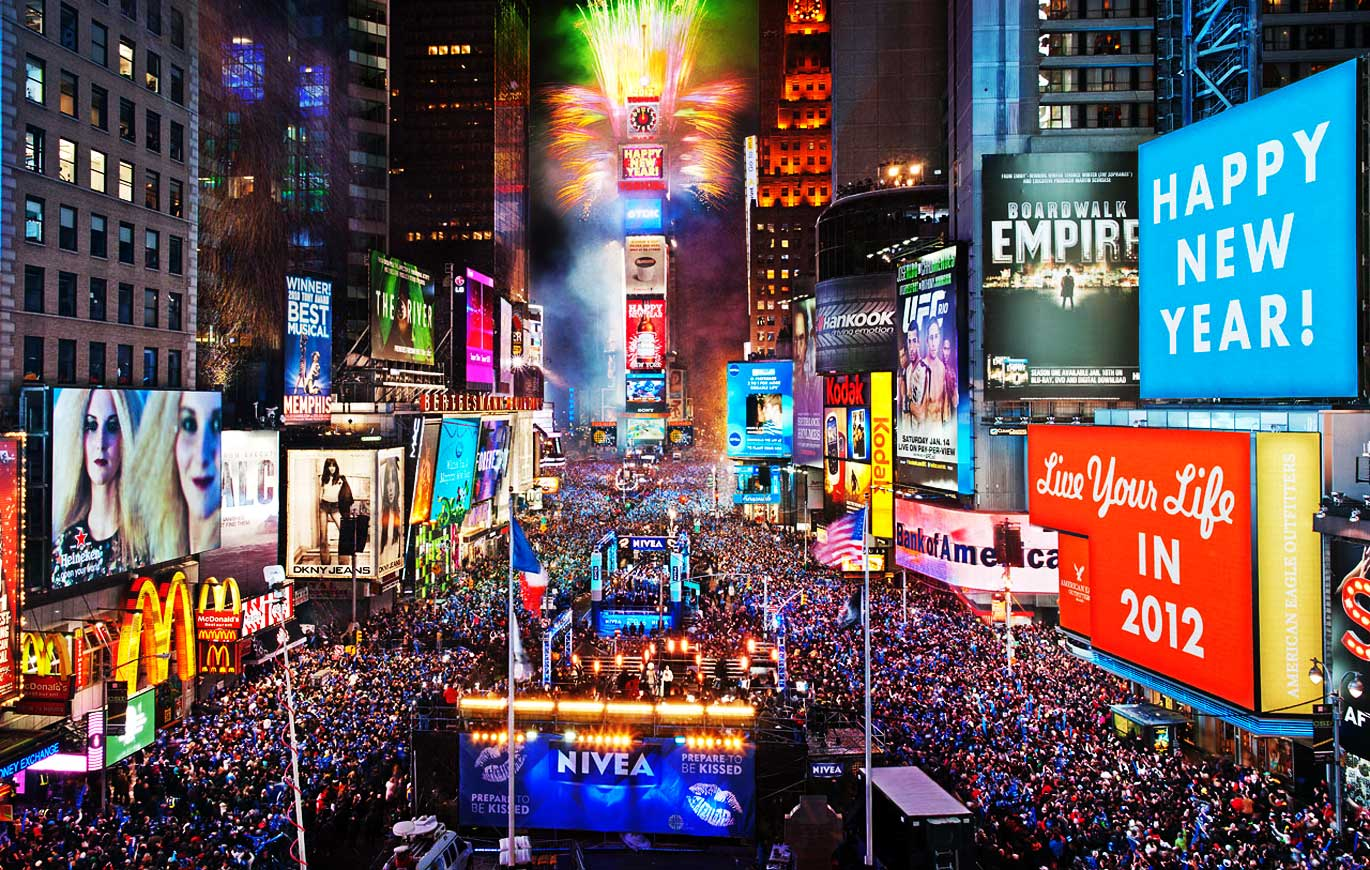
\includegraphics[width=0.5\textwidth]{./images/new_york_displays.jpg}}
  \hfill
  \subfloat[New York in the 60s]{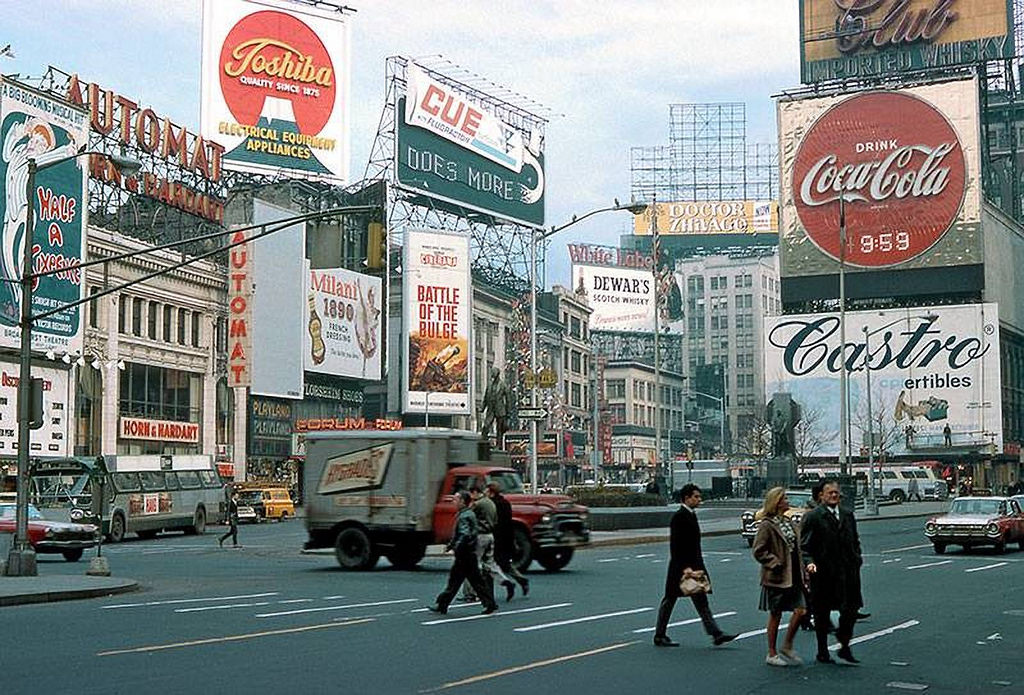
\includegraphics[width=0.46\textwidth]{./images/new_york_posters.jpg}}
  \caption{}
\end{figure} 

\subsection{Goal}
The goal of this project is to develop two new interactive displays application and a system to enable users preferences and supporting active and walk-by contact personalisation.

The architecture must provide a mobile application to manage users informations, access interactive applications and discover nearby displays using bluetooth beacons.

Since we are targeting a heterogeneous audience, the content must be easily accessible. So, we focus our attention to the UI design aimed to provide a natural flow of interaction between the system and each interactive application.

Moreover, the architecture must be scalable in order to allow future developers to extend our project by adding, for example, new applications to the displays. 

\subsection{Results}
With our project, we created a network that supports users personalisation into displays by developing a new architecture with two interactive applications.

The audience can see their preferences by just walk nearby a screen while interact with the mobile application. Also, informations can be retrieved directly from the display using a touch interface, For instance, is possible to see buses' schedules by clicking on a station.

In order to store the state of displays, applications and beacons, a \emph{MAP Provider} was developed. Also, it exposes a web socket is used to broadcast real time notification through all the system notifying the presence of a user near a screen.

The applications developed are \emph{Transport} and \emph{Upcoming Classes}. \emph{Transport} allows users to select their bus schedules as preferences and access useful content directly on the screen, like see directions from the display to the stations.
\emph{Upcoming Classes} shows the semester schedules supporting custom queries in order to discover specific content.

A colour based approach is used to identifier users' preference by only the creator. The user can select a custom colour in the mobile application that will be showed in the display.

\section{Architecture}
\subsection{Overview}
Our architecture is composed by three elements: Map Provider, and two interactive display's applications. We used a \emph{Micro Service} architecture in order to decomposing the application into different smaller services is that it improves modularity and makes the application easier to understand, develop and test. Each service is identify as a standalone web server.

In our project we deployed all the services on the same server hosted by the universities, but in a real world, they are usually physically separated

The components communicate using REST calls and Web Sockets that are proxied to the external world in order to serve all the applications from the same domain as is shows in Figure 2. Each of them expose an API that call be called in order to get the required data in JSON format.

The Map Provider stores the state of displays, beacons, users and the applications' informations in order to make them available for the system. A web socket is used to broadcast real time notification through all the clients in order to update their state.

We developed two display's application, \emph{Transport} and \emph{Upcoming Classes}, using the same common interface abstracting them into the \emph{Application Layer} (Figure 3.). Is it possible to individually add new applications by making them conform to our API interface for preference personalisation. Moreover, each application can be added from everywhere allowing developers to use their favourites technologies and hosting platform.
\begin{figure}[H]
  \centering
  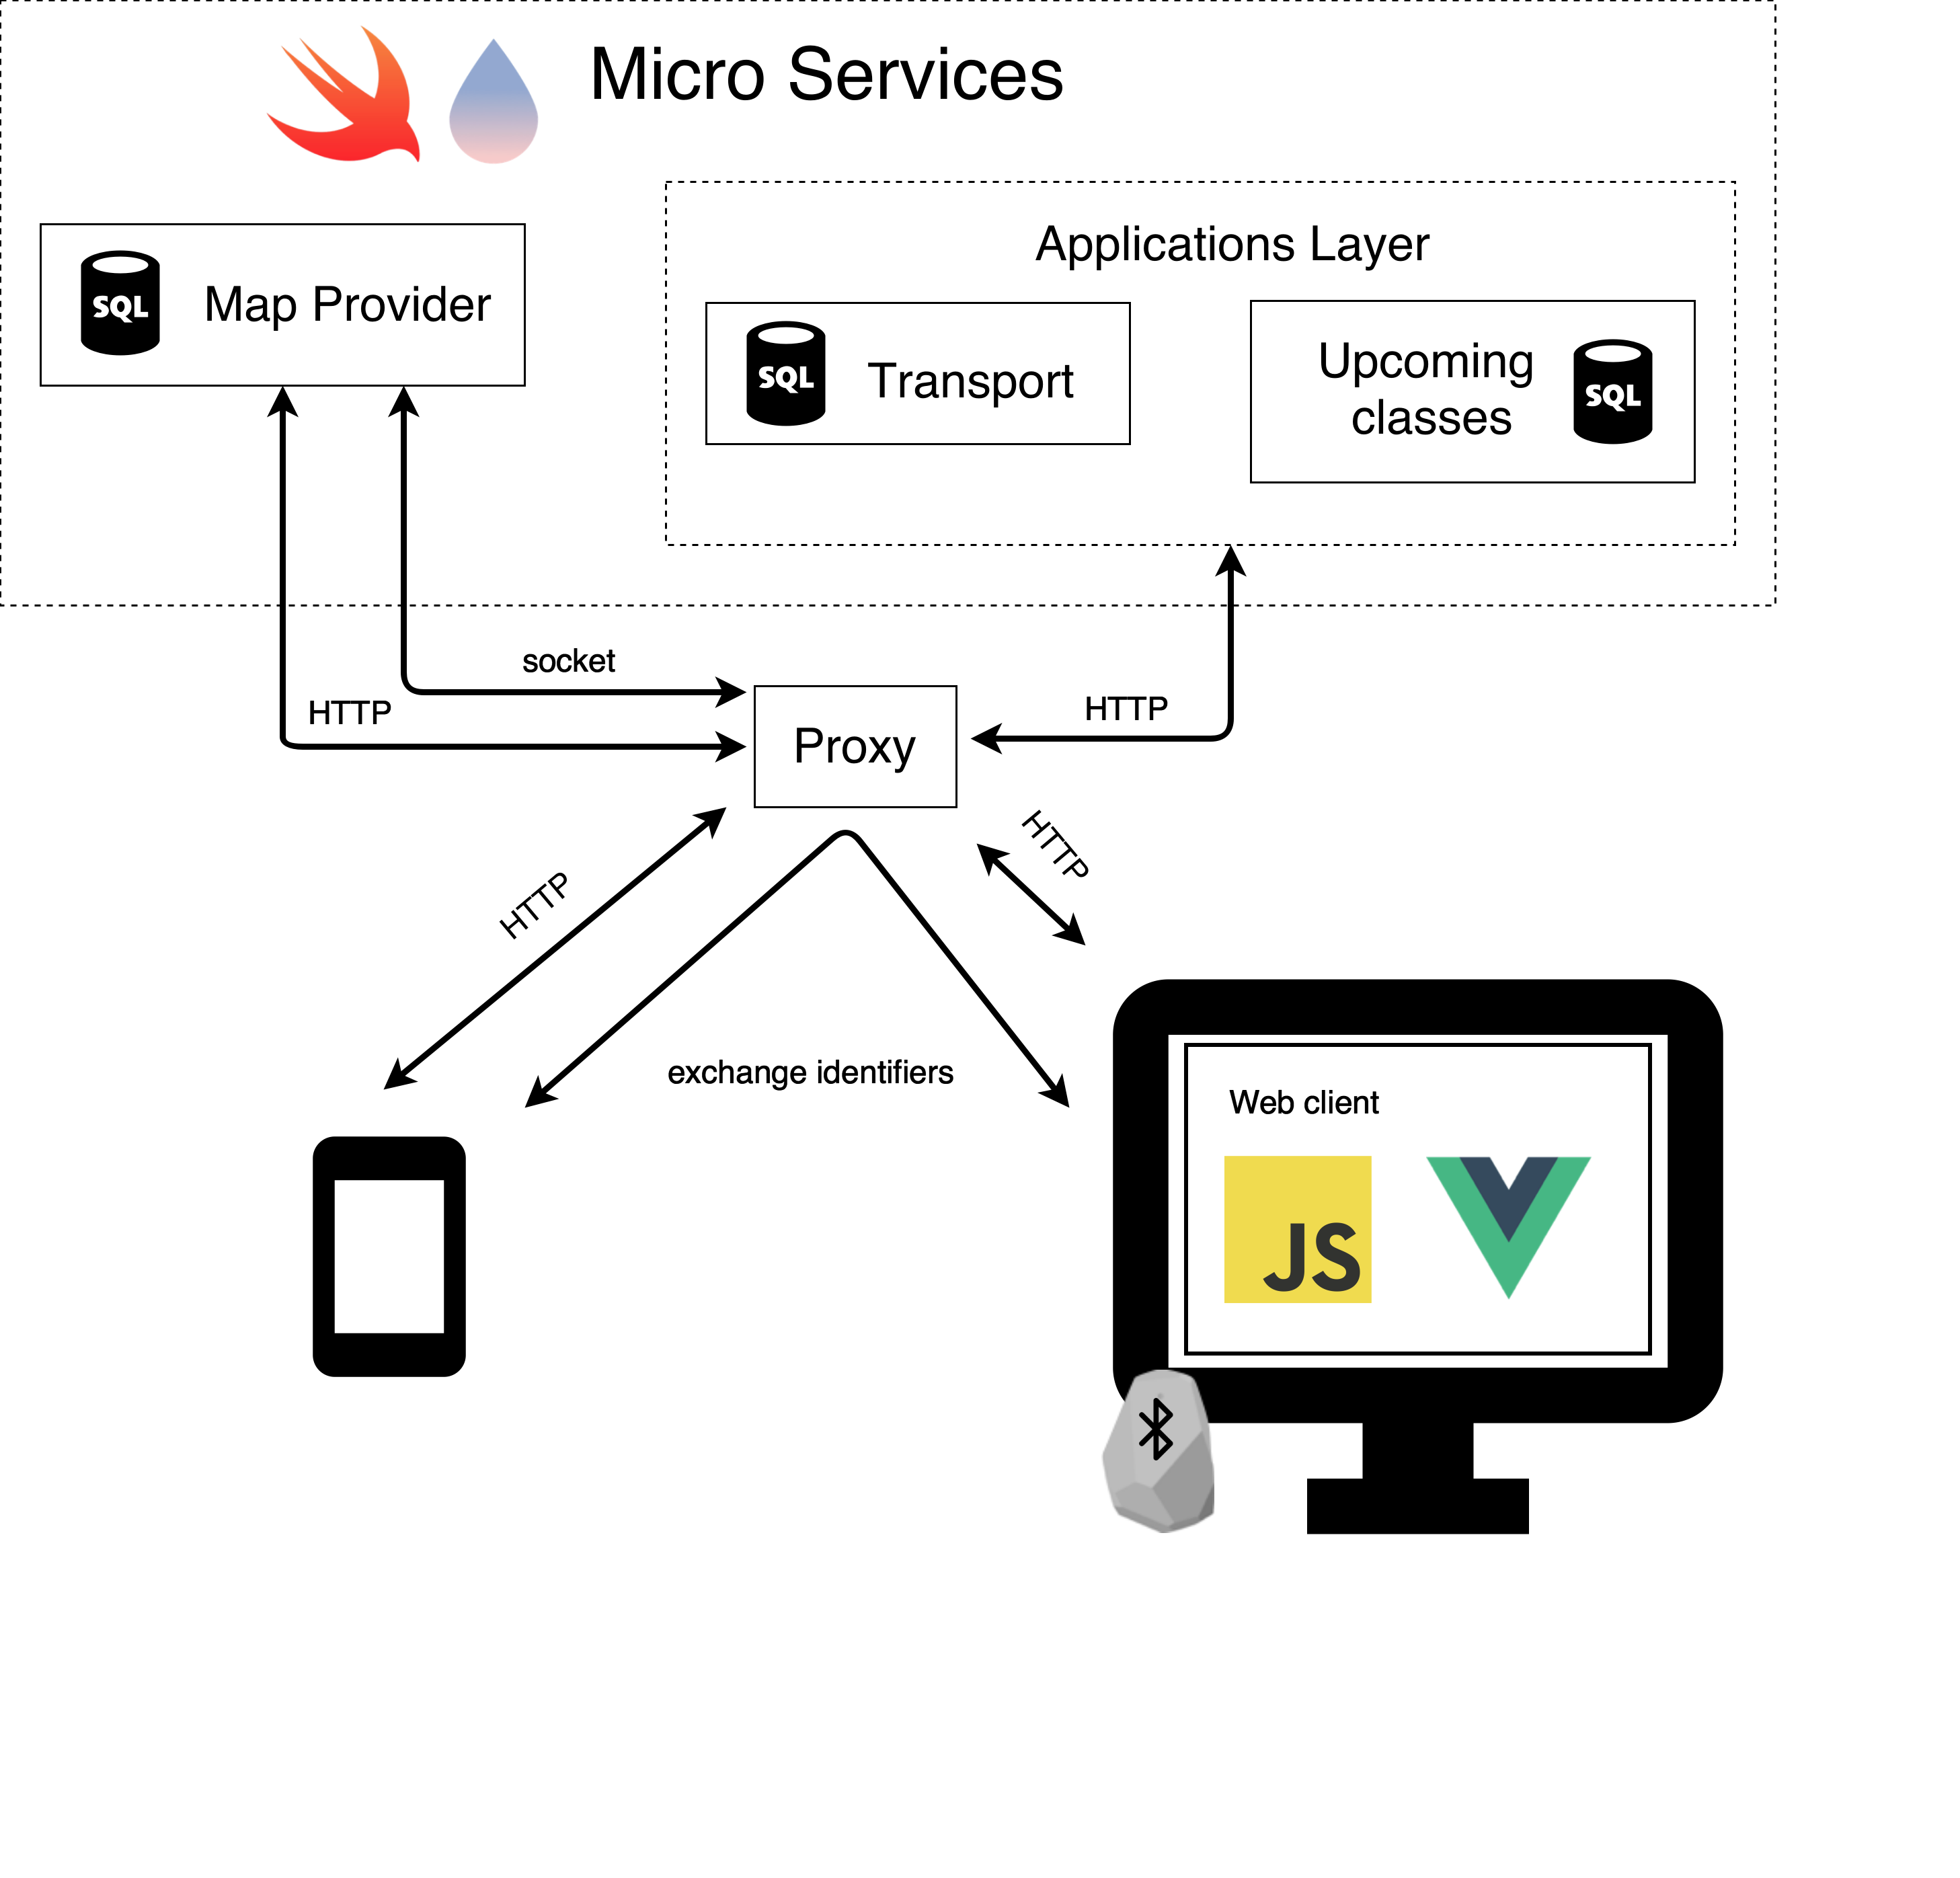
\includegraphics[width=0.8\textwidth]{./images/poster_image_1.png}
    \caption{Architecture Elements}
\end{figure} 


% TALK about the system that must be anynimous 
%
\subsection{Architecture Elements}
\subsubsection{Map Provider}
The \emph{Map Provider} stores in a database informations about displays, beacons and available applications in order to make it possible for the client access to the \emph{Application Layer} and have a global knowledge of the current network state. 

A many to one relation is created between the Display and the Application (Figure 4.) table, since, a single screen can run multiple application at the moment. In our project we limited to one main application for screen, but, using a responsive design approach, is it possible to maintain a pleasant look even if one is shrunk due to displays size limitation.

Since the \emph{Map Provider} allows to enable and disable custom services, a many to many pivot is used to keep track of local user's applications state. If an application is turned off and a user is near to a display running that application, then no interaction between the two will happen. In our design, this check, is done on the mobile application in order to send fewer information into the socket.

The physical device that make the in-walk communication possible is the bluetooth beacon produced. They are produced by Estimote. In order to link them to a screen, a many to one relation between Beacon and Display, since many beacons can be linked to a screen, but no the other way around. The model stores the beacon's mac address as unique identifier. These devices must be putted really close to the machine we want identify in order to increase the location accuracy. Moreover, thanks to our API design, they can be changed at any time by just send the correct request to the server.

A User model is stored with basic information such as email and favourite colour, they linked to Application with a one to many. 
\begin{figure}[H]
  \centering
  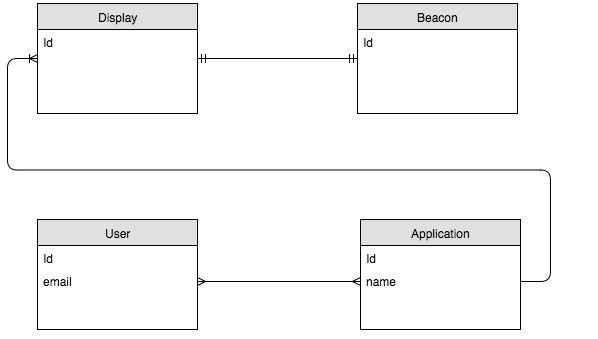
\includegraphics[width=0.6\textwidth]{./images/TacitaRelations.jpg}
   \caption{Relations in the Map Provider}

\end{figure} 

\subsubsection{Display Client}
In each Display runs a web browser in which applications, provided by each service server, are showed. For our project, we used a touch display provided from the university with a Intel NCU running Windows 10 connect to it. Our architecture can support any operating system, since it only needs a web client to run it.
  
 Since the applications are \emph{interactive} is it possible for the audience to interact with them using a touch interface to click on the application's page. The displays are \emph{active} elements that can interact with the world around them thanks to the bluetooth beacons that make them visible from the mobile application.
 
They are placed into key points of the university, such as, for example, \emph{mensa} or in entrance of the faculty. Is it very important to accurately study where to put them, since a poorly position can reduce the number of views.

Users can have a temporally and limited control on them by creating preferences that are showed when they walk-by.
Also, is it possible to dynamically change the running application by making a REST call to the \emph{Map Provider} that will notify the screen and make it update its state.


\subsubsection{Transport App}
The \emph{Transport} application allows users to navigate the nearby bus station and create preferences through the mobile interface. We decided to gather the data from the well designed Opendata API that allows to fetch all kind of transportation information, in our case we used only use buses.
However, due to the limit number of request we can made, fixed to three per second, and the necessity to have some custom endpoint, we cloned them.

We also have integrated Google Maps API into the screen's front-end. So, after fetching the exactly display's position thanks to web browser geo localisation, we can show the estimate time to get to a specific station by walk and the correct directions. With this informations we can give real time visible feedback on screen when it is going to be too late to catch a specific bus.

Since we are using a built in web browsers feature, we can easily scale our system. Image you need to move the display to one location to another, with our architecture there is no need to update its state into the server . Since the information is fetched client side, its position is updated as soon as it is moved, as well as with all the other functionalities related to it,  no external operation is needed.

Even if it can be argue that by cloning Opendata API we loose all information about delays, we notice that the delay field is always null. So, we have to assume that even them can not have access to such detailed information or it is not implemented yet.

For our project, we cloned them every 6 hours, but the schedule can be changed in virtual no time.

% say how ofter we clone them
% link to opendata
% put some pictures of the screen gui
% show some pictures of the preference flow
\subsubsection{Classes App}
The second application is \emph{Upcoming Classes}, it displays information about classes such as the course schedule for the next days. Is it possible to select preferences or to create queries for specific courses from the screen. All the courses are displayed into the calendar in the correct order supporting booth month and week view.

Similarly to the Transport application, we had issues with the API, in our case, provided by the University itself.
A single API call to know all the schedules takes more than $1500ms$ as showed in Table 1. It gets worse if you try to get all the courses for a faculty:
\begin{table}[h]
\centering
\begin{tabular}{|l|c|}
\hline
Request & Time \\\hline
http://search.usi.ch/api/courses/35255488/schedules & 1952ms \\
http://search.usi.ch/api/faculties/1/courses & 9294ms\\\hline
\end{tabular}
\caption{}
\label{table:usi_request}
\end{table}

Therefore they cannot be properly used in a real application. Even if, from the client, we always cache the request, we cannot avoid to wait for the first time. The reason why they are so slow is the response size. Their response is heavy due to a poorly model population; for each course that is sent back, tons of unused field are provided. Also, by inspecting a response for a class schedules, we can notice the same huge course object appears, unnecessary, for each schedule object.
Therefore, again, we needed to clone all the API in order to just sent the right amount of information, by doing that, the previous schedule request now needs just $18$ms. Table 2 shows these results.

\begin{table}[h]
\centering
\begin{tabular}{|l|c|}
\hline
Request & Time \\\hline
http://tacita/classes/api/course/246/schedules & 18ms \\
http://tacita/classes/api/faculty/1/courses & 1000ms\\\hline
\end{tabular}
\caption[Table caption text]{}
\label{table:classes_request}
\end{table}
The display's front end application is divided into two main part easily identificable, the calendar and the query engine next to it. The calendar is create using \emph{fullcalendar} jQuery library that does all the dirty work of render and setting up all the events into the corrects slots. 
The courses can be selected thanks to the query engine on the right part of the screen. As soon as the user clicks on the button representing the faculty, it is guided in order to create a valid query using a step by step approach; even if it may be not the faster way, it is the safest since no wrong request can be generated. The procedure is shows in the following storyboard:
% aggiungi storyboard classi

As we did for the Transport Application, we also created a smart phone interface in order to create, remove and edit preferences. Since the interface is always the same we decided to also decide to keep the same design for consistency reason.
% show transport app similar to this one
\subsubsection{User}

The User has a fully active role, he is the trigger of the whole system; without him, the network has not reason to exits. He uses his smartphone in order to access the front-end application exposed by the \emph{Appliction Layer} through the smartphone platform.

By using it the User can selects his custom settings in order to quickly identify his information on the screens.
In our design, a favourite colour can be selected in order to filter fast the owned content and gaining anonymity, since nobody else can know who is linked to a specific colour. Also, colour base information can be identify really fast by just watching the screen.
This application will be deeply analized into the next sections, but, from a user point of view, it is the door to access the whole array of services.

We talked about the User as a \emph{trigger}, it means that, with his physical being, it \emph{triggers} actions; actions that are universally recognisable by our architecture. While walking near a screen, the architecture, thanks to bluetooth beacon that map them in the space, and, thanks to the smartphone application, can detect the movement show the personalised content into the screen at the right time. For the client, this is very convenient, since no other interaction is needed at all. One challenge we encountered was to make sure that the required content is showed in the correct time because, if the architecture is unreliable for the user then nobody will trust to use it.
 
 
\subsection{Architecture Interactions}

In the previous part we define in detail each element of our architecture without giving a global overview of how each parts collaborate with the all system. In this section we are going to analyze all the interaction, especially between user and display, showing and explain each message that the entities exchange in order to communicate.

From a User point of view, the first actions that can happen is walking into a display.

 As soon as the mobile application detects the beacons, it gets a list of them sorted by distance (action $1.$ of Figure 4). The first one is fetched and its id is used to make a request to Map Provider ($2.$) in order to know which display is associated with it. If there is one, a message containing user's id and display's is pushed into the socket ($3.$) only if the screen application is enabled. An example message:
 
 \begin{lstlisting}
{
  action: 'USER_NEARBY',
  payload: {
    user_id: '1',
    display_id: '1'
  }
}
 \end{lstlisting}
 
When the display receive the notification, it checks if it has the same id. If it gets the user's preference from the back-end running application ($4.$). Finally, the user's content is showed into the screen ($5.$).

Similarly, when a user walk away it lost its connection with the beacon and a new message is pushed into the socket in order to remove its preferences from the display.
 \begin{lstlisting}
{
  action: 'USER_EXITS',
  payload: {
    user_id: '1',
    display_id: '1'
  }
}
 \end{lstlisting}

To avoid processing the same information two or more times, the displays uses a in memory cache. Also, a life duration is set for each of them in order to remove them if no exit event is detected.
\begin{figure}[H]
  \centering
  \includegraphics[width=0.5\textwidth]{./images/elements_interactions_user.png}
  \caption{Architecture Interactions, User point of view}
%    \subfloat[Display interactions]{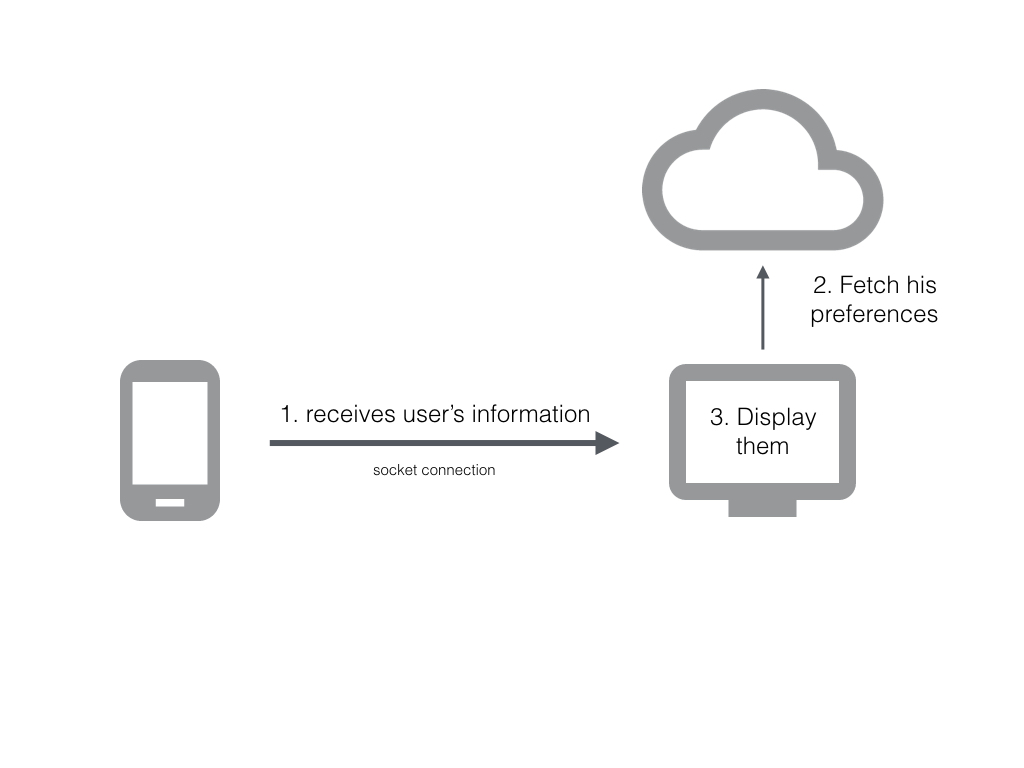
\includegraphics[width=0.5\textwidth]{./images/display_interactions.jpeg}}

\end{figure} 
When the display's web client is connect to one of the applications (action $1.$ Figure 5), it does some initial setup ($2.$). Depending on the local case, it may ask for the geo localisation, used in the \emph{Transport application} or create some data structures. After the boot phase is done, a request for the data is made to its provider in order to show informations ($3.$).
In the mean time, the screen sends the applications that its running to the \emph{MAP Provider} ($5.$) in order to update its state. Then the \emph{Provider} broadcast to all the clients the new informations using sockets so each element has a global real-time view of all the displays state. In our project, the mobile application, when it receives such information and if the new application running is enabled, it sends again the user's identifier in order to show the personalised content into the new application without reload the view.
\begin{figure}[H]
  \centering
  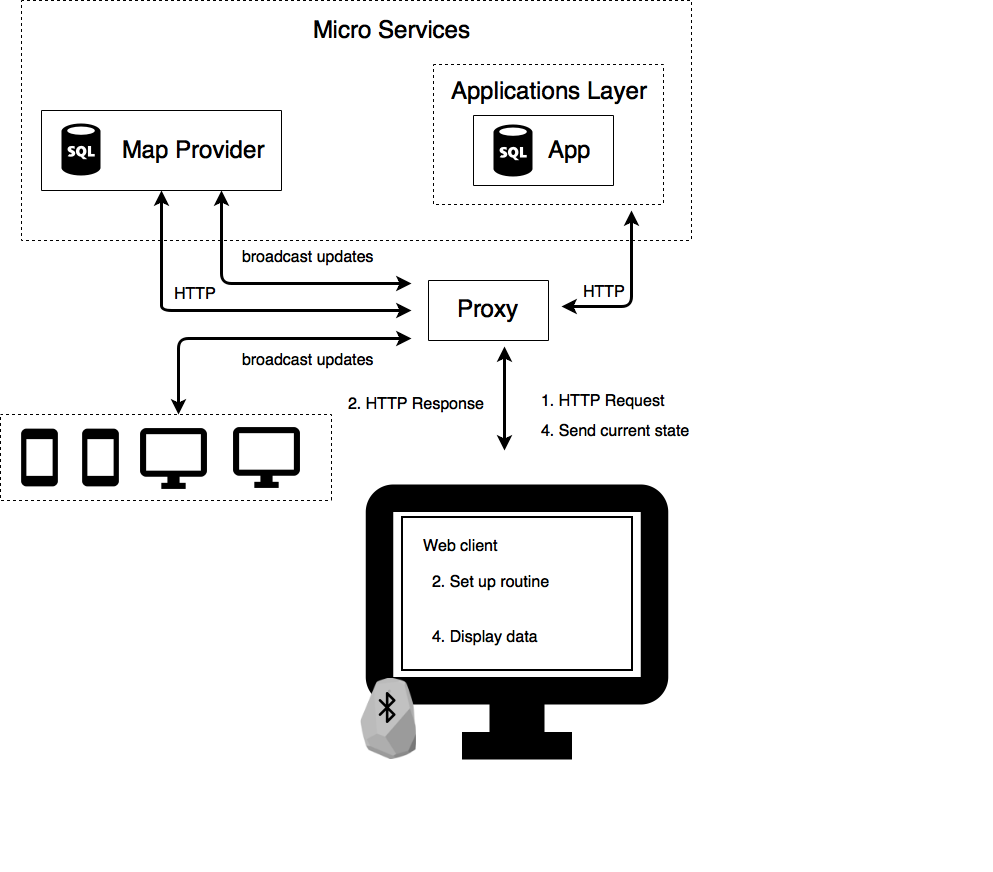
\includegraphics[width=0.5\textwidth]{./images/elements_interactions_display.png}
  \caption{Architecture Interactions, Display point of view}
%    \subfloat[Display interactions]{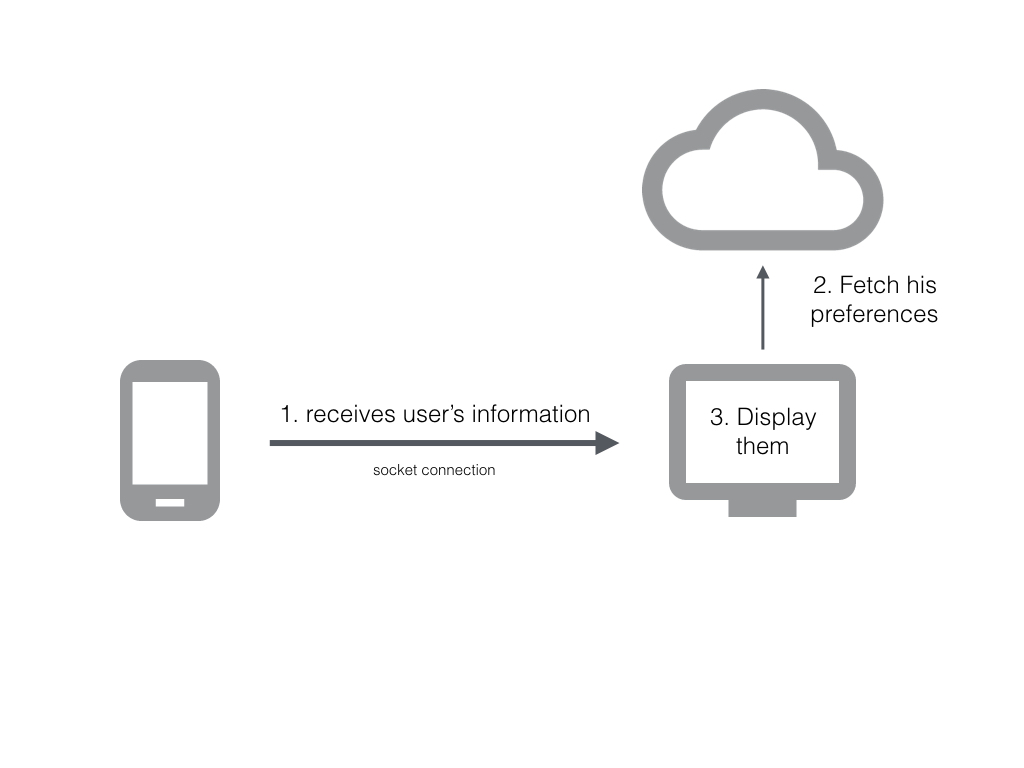
\includegraphics[width=0.5\textwidth]{./images/display_interactions.jpeg}}

\end{figure} 
To each screen is associated an unique id. Therefore, before deploy a display, it must be create a new entity in our database by making the correct request to the \emph{Map Provider}. The id is passed to the display's client by adding it in the end of the url that is processed by the front-end software.
\subsection{Architecture Technologies}
In this section we talk about the technologies that we used for the back-end and the front-end. For this project, we choose the latest technologies and programming languages in order to provide a service that will last without being obsolete in a long term.
\subsubsection{Back-End}
We firstly started to develop the first application using Django, a widely used python web framework, but we encored problems with web socket that were not supported "out of the box".
So, we decide to completely switch both language and framework by choosing Swift 3 and Vapor.

Swift is a "powerful and intuitive" open source programming language developed by Apple in 2015 for booth MacOs X and Linux. It is a Protocol Oriented Programming Languages.
%\\
%\emph{A protocol defines a blueprint of methods, properties .. The protocol can then be adopted by a class, structure, or enumeration - Apple}

Unlike classes, the fundamental of Protocol Oriented Programming, POP, is Value Type encouraging flat and not nested code. This benefit is reflected into its performance and flexibility.
The syntax is concise yet expressive, it uses labels and spaces to improve the code readability making possible to write complete sentences only with code. Apple wanted to create a product that was at the same time, feast and beauty.

After selecting a programming language, we need a framework to create our applications. We choose Vapor for the job; a powerful, beautiful and easy to use MVC framework to build web servers. In our project it powers all micro services.
Vapor is easy to start with thanks to the clear APIs that, not also speed up the developer work, makes the code more maintainable and more understandable. One of his strength point is the performance inherited from Swift. \subsubsection{Front-end}
In order to archive the best results in term of scalability and performance we choose Vue.js as main front-end framework. Vue.js is a library for building interactive web interfaces, it uses web components to provide a convenient way to organise an application by decoupled its element into blocks.
A web component is similar to a Object Oriented programming classes, it encapsulate all the logic behind a certain functionality of the application. In Vue, a component, in formed by three parts: template, script and style.

The template allows the developer to write html and include variables, conditions and loops. Also, thanks to build in loaders, is it possible to easily use any pre-processing html library such as Pug.
The second part is the core of each components, the script. As the name may suggest, it is the code part. Each component expose a javascript object allowing Vue to grab it and render it in the proper way.
The last tag is were is possible to style a component using CSS, as before, it is tremendously easy to use Less, Sass and other css-processors.
One of the main advantages of Vue over other front-end framework is \emph{reactivity}. Reactive programming is an synchronous programming paradigm concerned with data streams and the propagation of change. It uses Observers in order to trigger events every time a change of state is detected; therefore Vue can automatically call a render only in the part that was actually mutated minimising the DOM access and increasing speed.
A deeply comparison with other frameworks can be fount at: https://vuejs.org/v2/guide/comparison.html.
%\begin{figure}[H]
%  \centering
%  \subfloat[Vue.js vs other popular libraries]{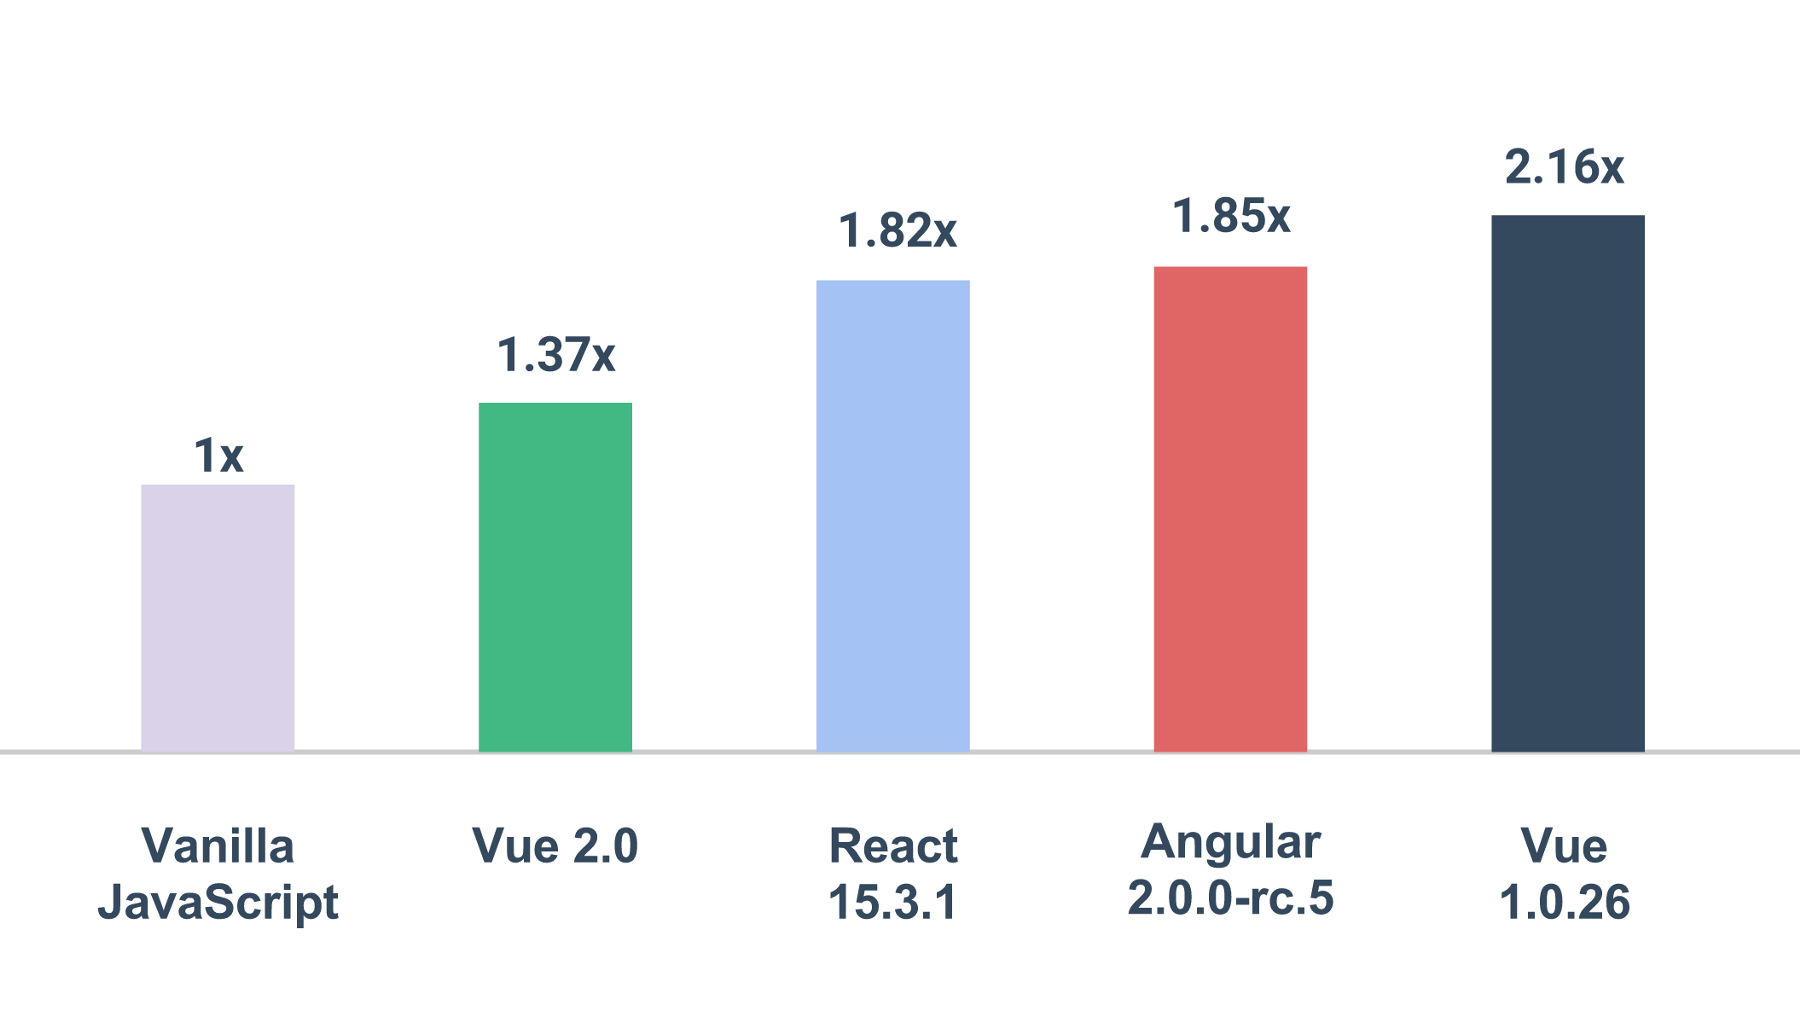
\includegraphics[width=0.5\textwidth]{./images/vue2_benchmark.png}}
%\end{figure} 
As we said, each component represent a feature, a part of the web application; it may happen that one of them need to communicate with another, maybe after a change of state or a user event. In order manage the data flow we used the Flux pattern. The mainly idea behind this pattern is that the state can be mutated thought actions that are reduced into the stores. It is composed by four parts: Dispatcher, Store, Actions and View.

The dispatcher is a singleton that receives them and dispatches to every stores that have registered with it; its important to highlight that every store receives every action.

The Store is only source of truth in the applications; it holds its state and manage the logic behind it. The data must only be mutated by responding to and action by emitting a "change" event.

Actions are the internal API of each application, they define all the possible interaction that may happen. They are plain javascript object composed by a type field and some data.

Views displays store's data; in our application, a single view is a Vue component.

Even if there already exist a fantastic Flux library, Vuex, for Vue created by its author, we decide to create a new one from scratch. Our library, called Flue, aims to provide a better object oriented approach than the existing one. You can find examples and documentation at our Github repository: https://github.com/FrancescoSaverioZuppichini/Flue.

\begin{figure}[H]
  \centering
  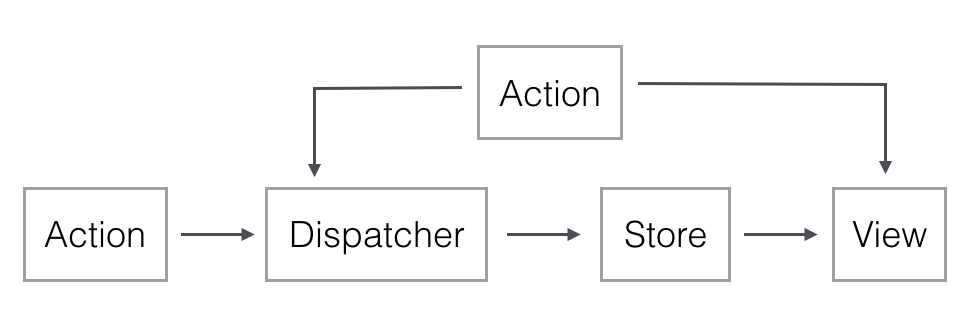
\includegraphics[width=0.5\textwidth]{./images/flux_data_flow.png}
  \caption{Flux data flow}
\end{figure} 
\subsection{Architecture Scalability}
Scalability is the ability of a system to grow larger with minimum changes. In the previous sections we often talk about how some design choices lead to an improvement in term of scalability. In our specific case, our system can change very quickly at any moment: just image if the provided buy new displays or new applications are available.

In order to make it possible to deploy independently from the network a new application, we abstract the its concept creating a layer of services that can be expanded very easily. The developers can create a new applications by just creating a web server being conform to our generic interface and expose his url.

Another possible problem that can may appear is when a display is moved away. We explained before how each screen, when its connected, fetch its position and use it in order to communicate with Google Maps API to show real direction indications. If such problem appears, very easily, the provider just need to refresh the screen and the front-end software will automatically update itself.

Also displays can be removed or added by simply using \emph{Map Provider} REST API. Imagine a screen breaks, then the associated beacon can be moved to another screen or the display may be replaced. The last case is the easiest, since we can just turn on the screen and use the last display's id, if no new devices is available then the beacons can be quickly be linked to the a new screen.
\section{Design Interface}
Our application is exposed to a heterogeneous audience, therefore a clear and effective interface is mandatory to ensure a global usability. 
We have also to provide a no blocking content flow in the displays' applications, meaning that an interaction should not prevent, or block, another.
Moreover all the state changing must be displayed using design techniques, such as well targeted animation, in order to make the user understanding what is happening around him.
We decide to follow a \emph{content first} strategy by making the content clear and visible using a minimalistic approach; no unused element is present in any application. We choose cards as only way to organise information. A card is a sheet of material that serves as an entry point to more detailed information proving a convenient way to display content composed of different elements.
% qualche efoto di card
\subsubsection{Display Applications}
The main challenge was to design for a big touch interface. We started by keeping in mind that every information must be quickly reachable and accessible; the user must understand in a fraction of second what he needs. By keeping that constrains in mind.
Our design process starts with wireframes; representin the skeletron of the application exposing its main functionalities. They are terribly useful to get a first general look of what the application is going to be. For what It concern the Transport service, we begin by discard every not necessary element following, as we said, a minimilistic approach. In the following picture you can see the first wireframe's muck up and the final product
\begin{figure}[H]
  \centering
  \subfloat[wireframe]{\includegraphics[width=0.43\textwidth]{./images/transport_wireframe.png}}
  \hfill
  \subfloat[final product]{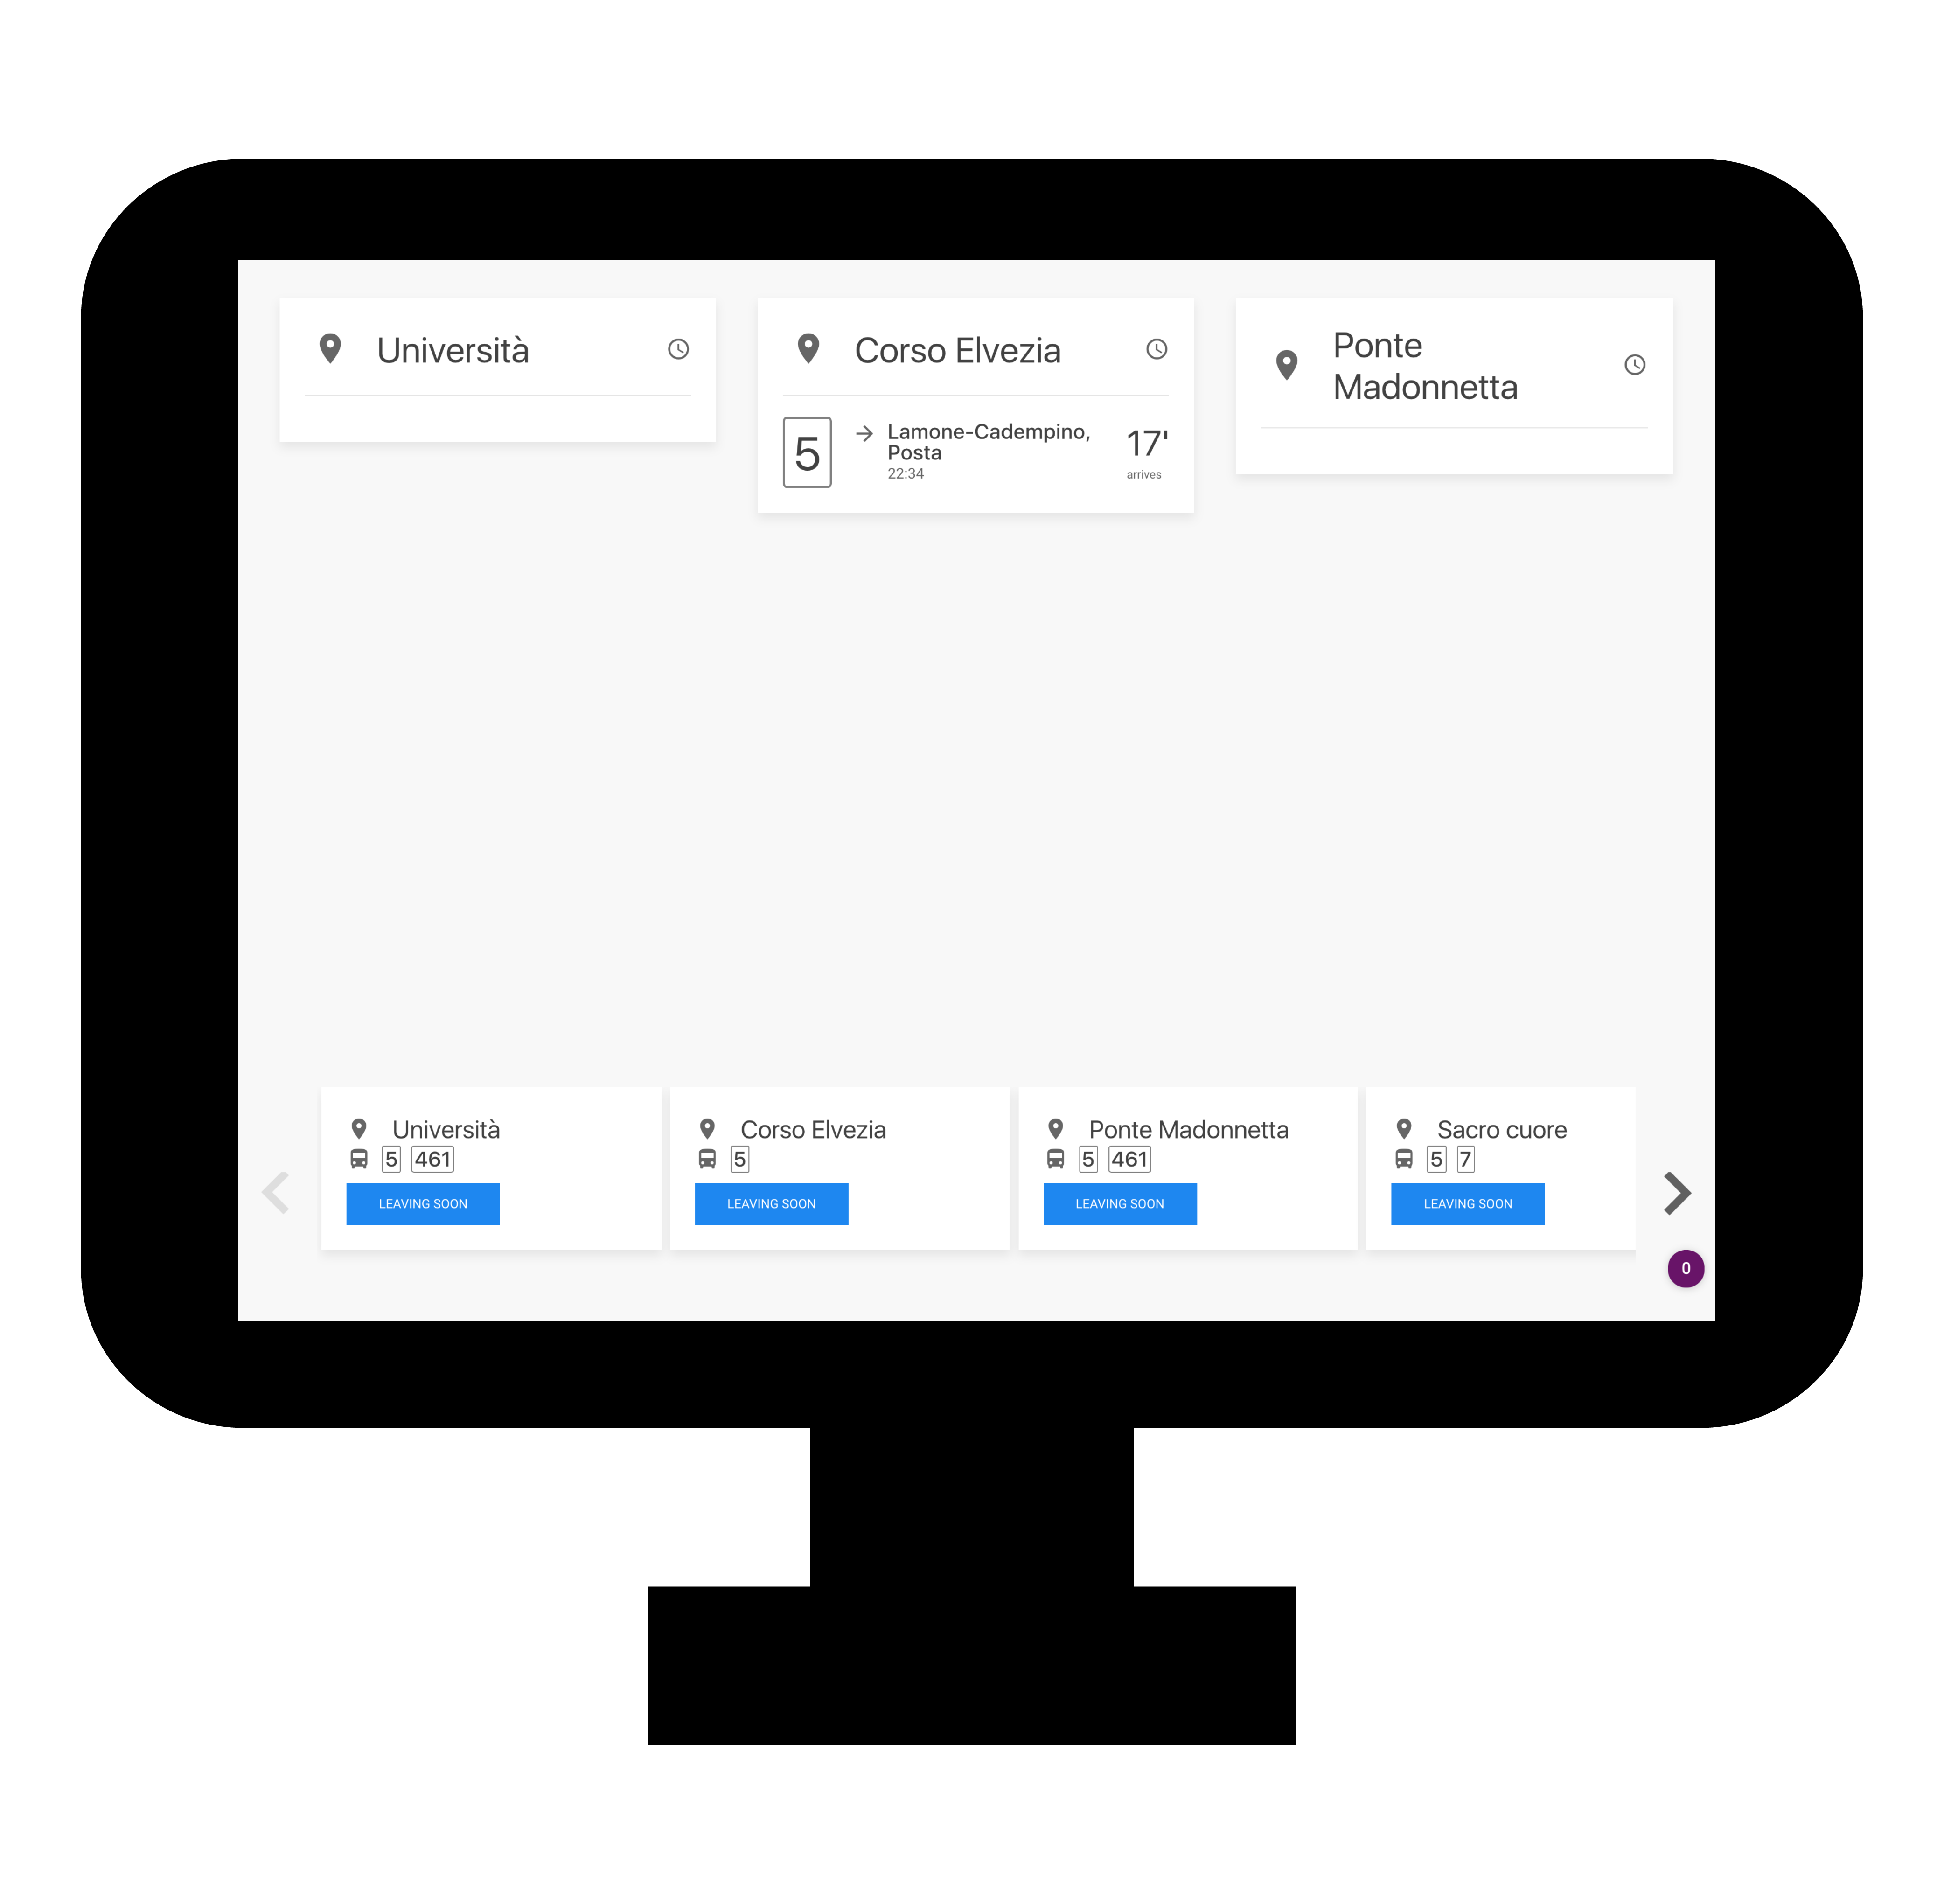
\includegraphics[width=0.53\textwidth]{./images/transport_application}}
  \caption{Transport Application}
\end{figure} 
If you look at the left image you can notice that all the functionalities are intuitively recognizable. As we said, our design, must be carefully studied for big display; we focus on the interactive part.
At the bottom of the application there is a carousel used to change station on the fly. All buttons are big enough to be easily be used from everyone without any problems.
Moreover, we used animation to increase the user experience; when a station is selected is pushed on the right part using a slide in animation making more visible. Also, a open station shakes when a user try to open it again giving a strong visible feedback of where it is on the display. 

In the Class application we used the same approach, we started by sketching the wireframes and defining the main functionalities. In this specific case, we need two components: a Calendar and a query engine to search courses. 
\begin{figure}[H]
  \centering
  \subfloat[wireframe]{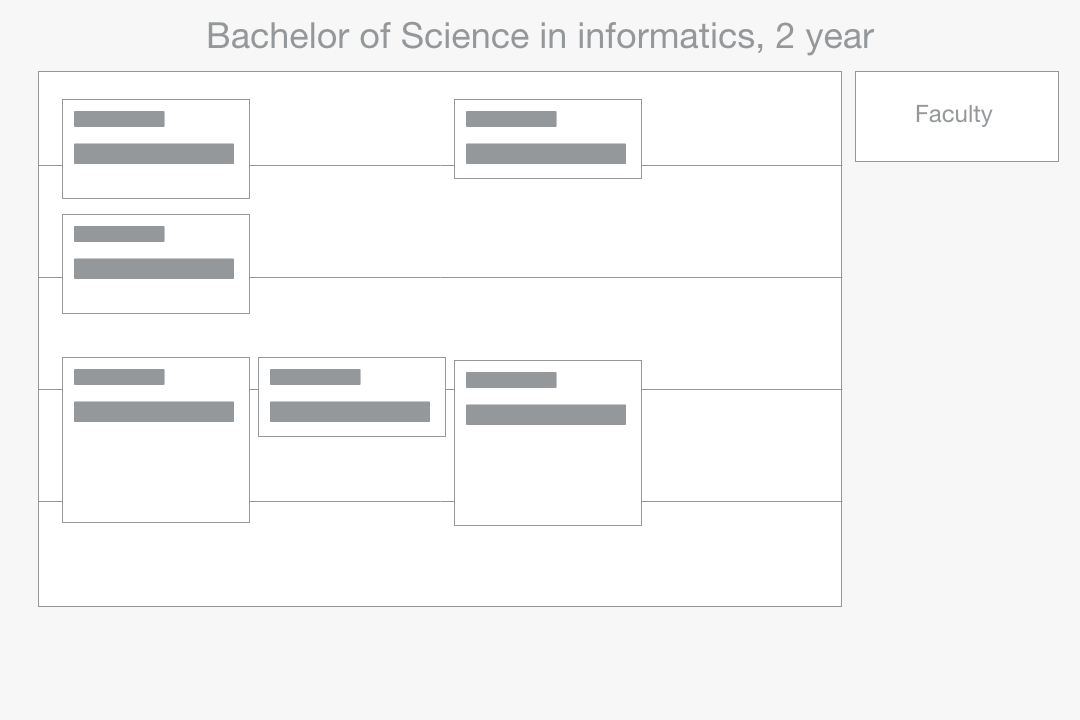
\includegraphics[width=0.43\textwidth]{./images/classes_wireframe.png}}
  \hfill
  \subfloat[final product]{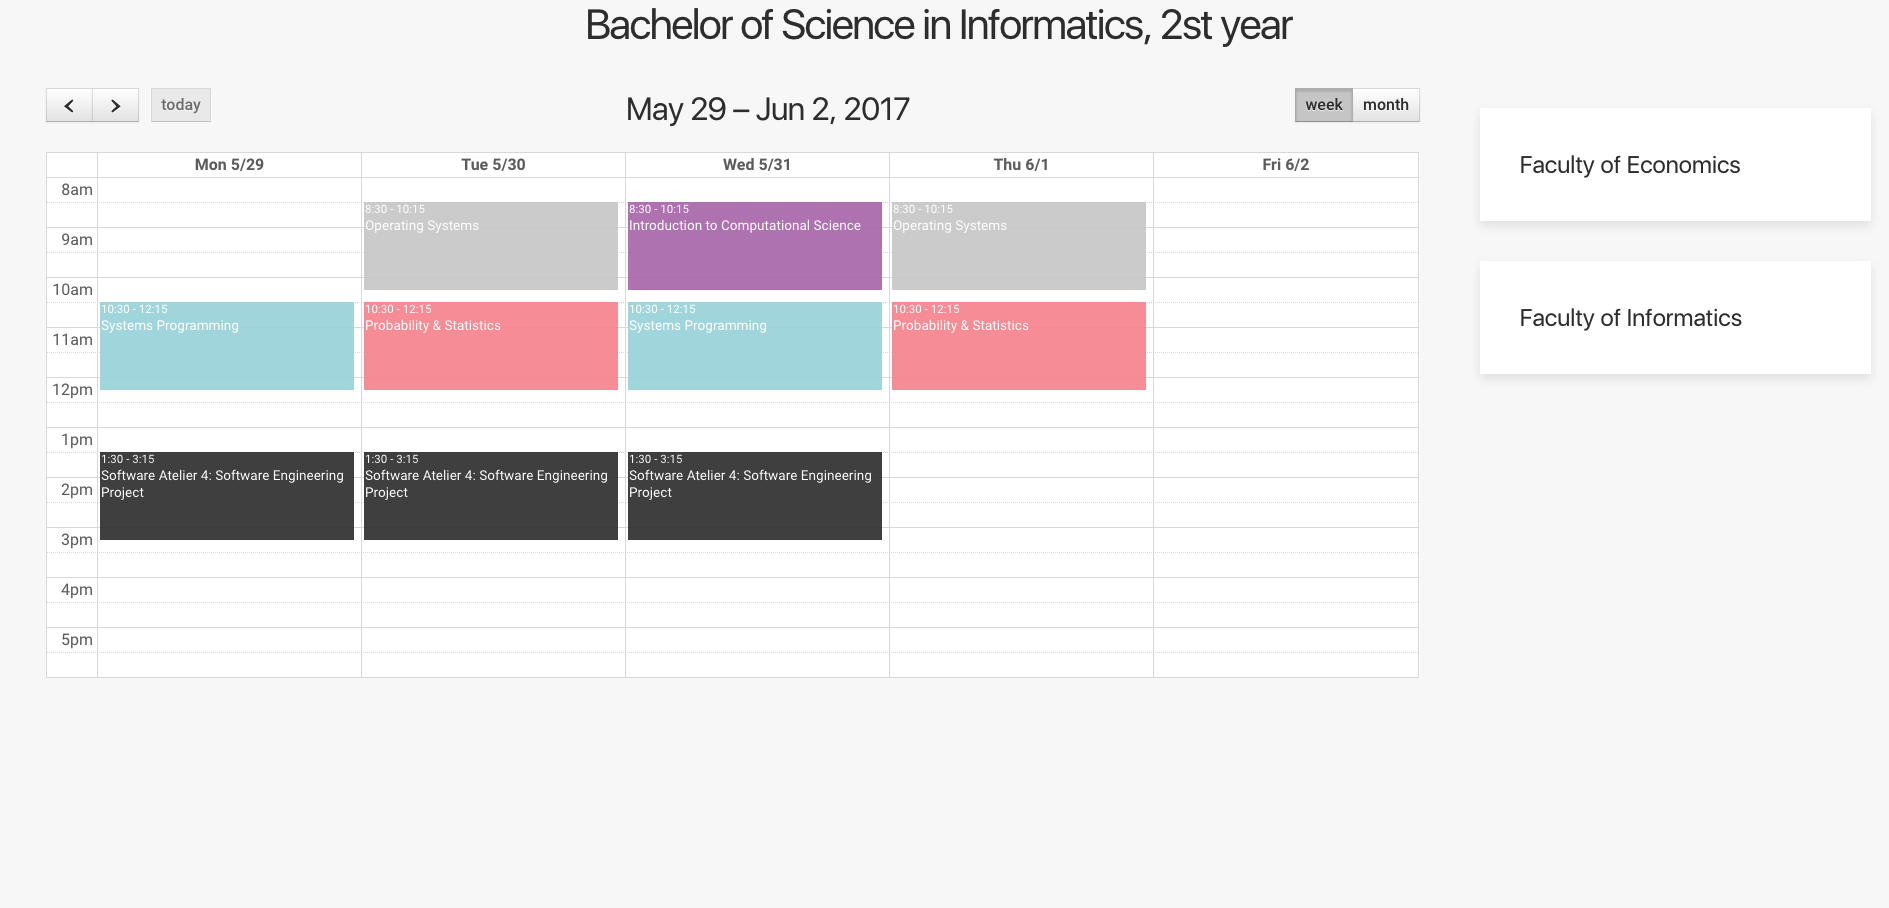
\includegraphics[width=0.53\textwidth]{./images/classes_application}}
    \caption{Classes Application}
\end{figure}
\subsubsection{Smartphone}
As we have explained before, we develop an smartphone application called \emph{Tacita} in order to organize the user interaction with the display. We design it from sketch to be accessible for everyone from everywhere. 
Logically, in main page of the application is possible to see and enable all the existing application exposed by the \emph{Application layer}. Since we wanted to provide a more comfortable user experience we added skeletron loader instead of a classic spinner; therefore, in case of slow internet, is possible to 'guess' the content of a page. Figure 9 shows this strategy. As you may notice, is it easy to understand how the content is going to appear on the application. We took advantages of such design pattern in almost all of our applications.
%\begin{figure}[H]
%\centering
%\subfloat[Loading]{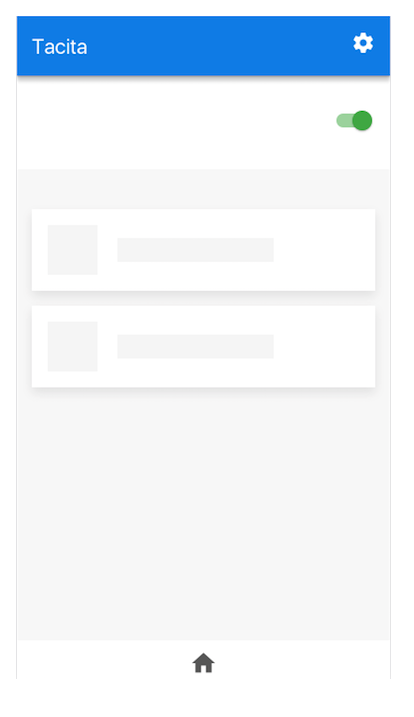
\includegraphics[width=0.4\textwidth]{./images/tacita_skeletron}}
% \subfloat[Finish]{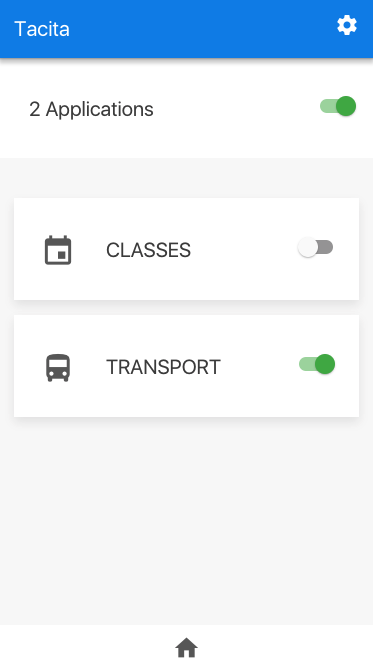
\includegraphics[width=0.4\textwidth]{./images/tacita_main}}
%\caption{Skeletron loading}
%\end{figure}
\begin{figure}[H]
\centering
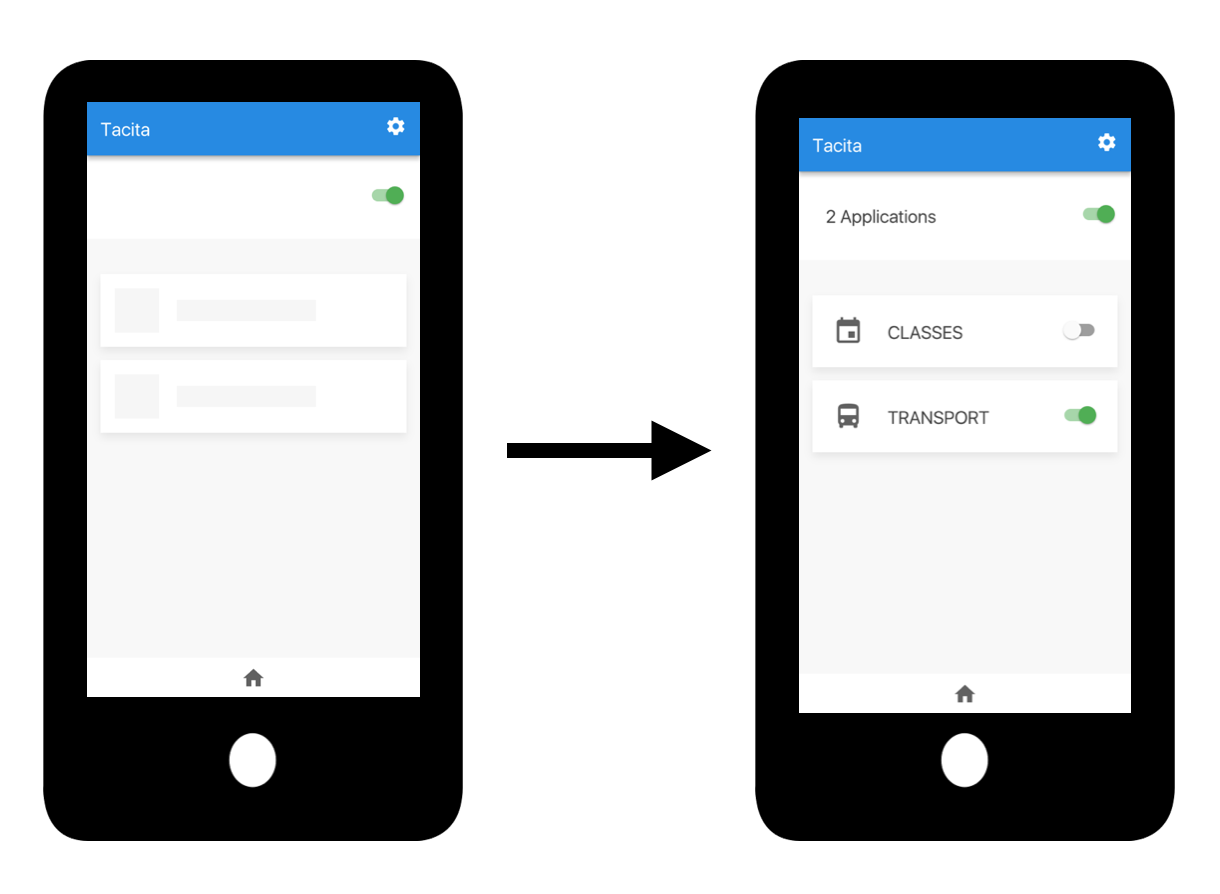
\includegraphics[width=0.5\textwidth]{./images/smartphone_loading_applications}
\caption{Smartphone home page}
\end{figure}

For each application a convenient toogle button is added to enable and disable it with just a click. If a user wish to enable/disable all the applications in one shot, the main button at the top can be used. If a provider decides to add a description for the application, then it is possible to read it using the arrow at the bottom of each card.

In figure 10 is present the view changes that occours when a User walk nearby a screen.A float button pops up making the displays page avaliable. These buttons represent a great way to quickly add a functionality to a view, we decide to create a pulse animation in order to make it even more visible for the user. Since we are using socket connection, if the display changes the running application, the client will be notified

\begin{figure}[H]
\centering
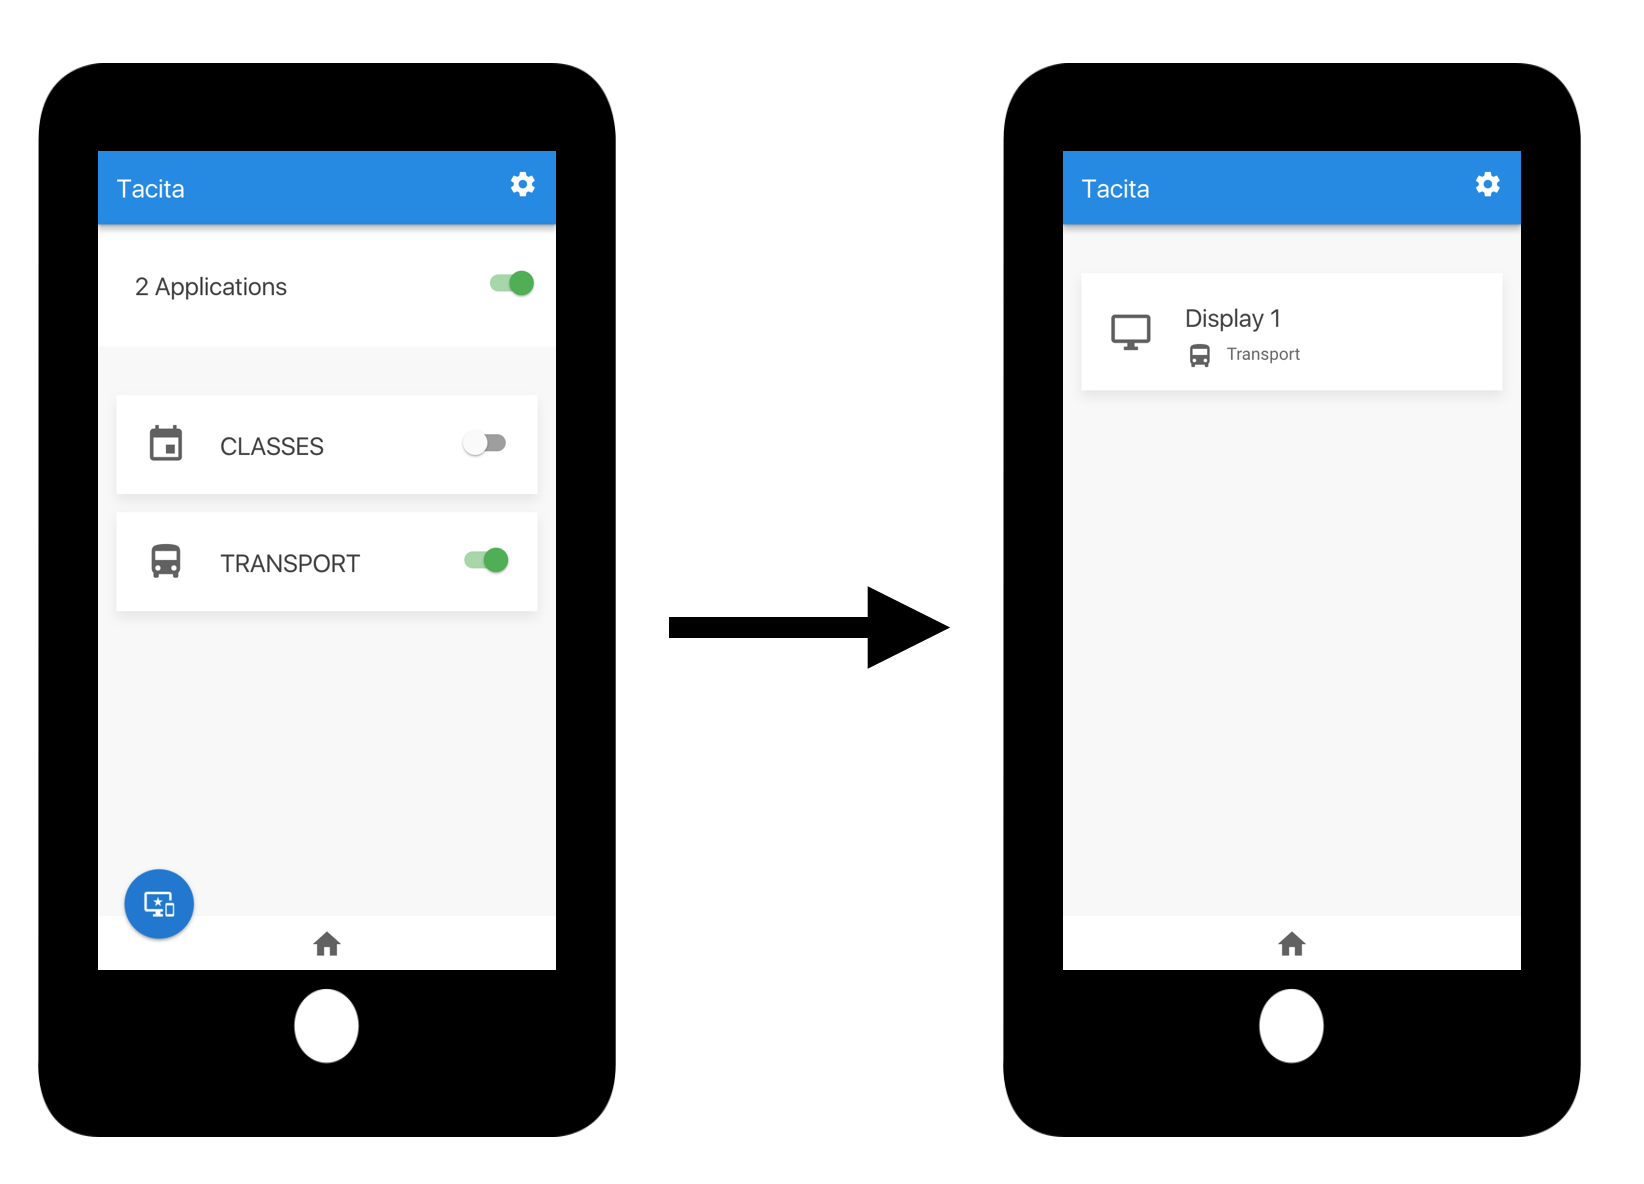
\includegraphics[width=0.5\textwidth]{./images/smartphone_displays}
\caption{Display found}
\end{figure}
As we said before, We also provide a convenient way to select a custom personalisation. We choose a colour based approach in order to highlight the visibility of a own content. The user can pick up a colour from the wheel and use it to find his preferences on the screens. Moreover, our system can easily support any other identifier such as username or avatar.
\begin{figure}[H]
  \centering
  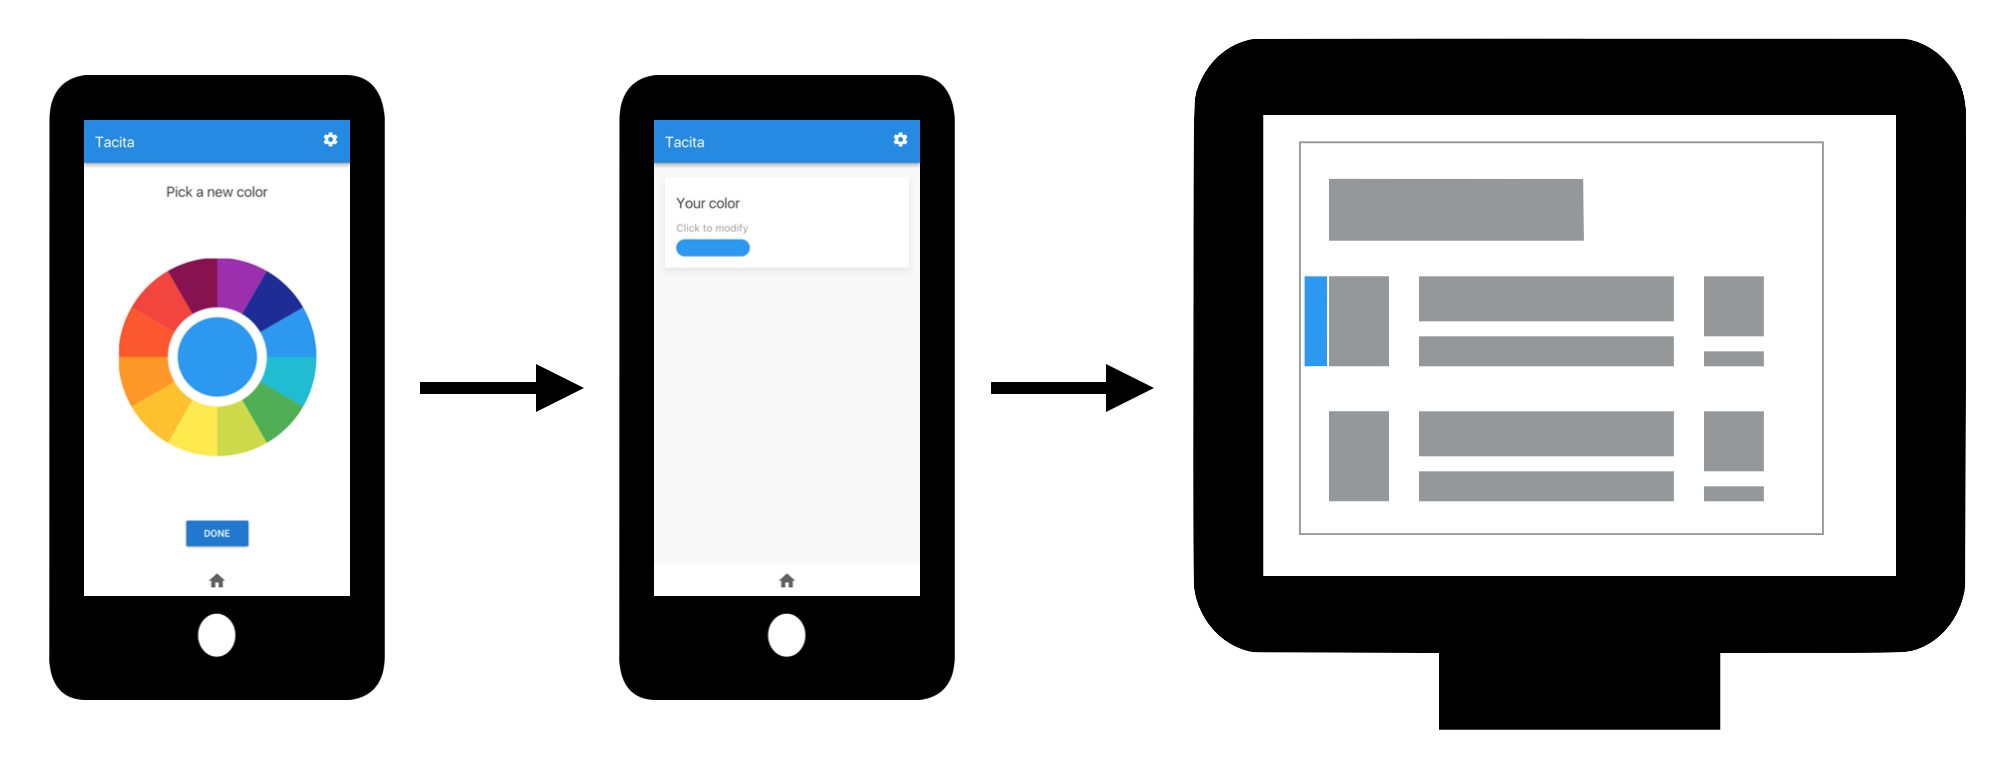
\includegraphics[width=0.7\textwidth]{./images/smartphone_color_preference}
  \caption{Preference on display}
\end{figure}
In this example, the User selected a "blue" colour as identifier of his preferences. In figure \emph{u} you can see the actually final result on the display, a little label is added on the left part of the selected buses. If one of more users walk in, then the label is splitted.
\begin{figure}[H]
  \centering
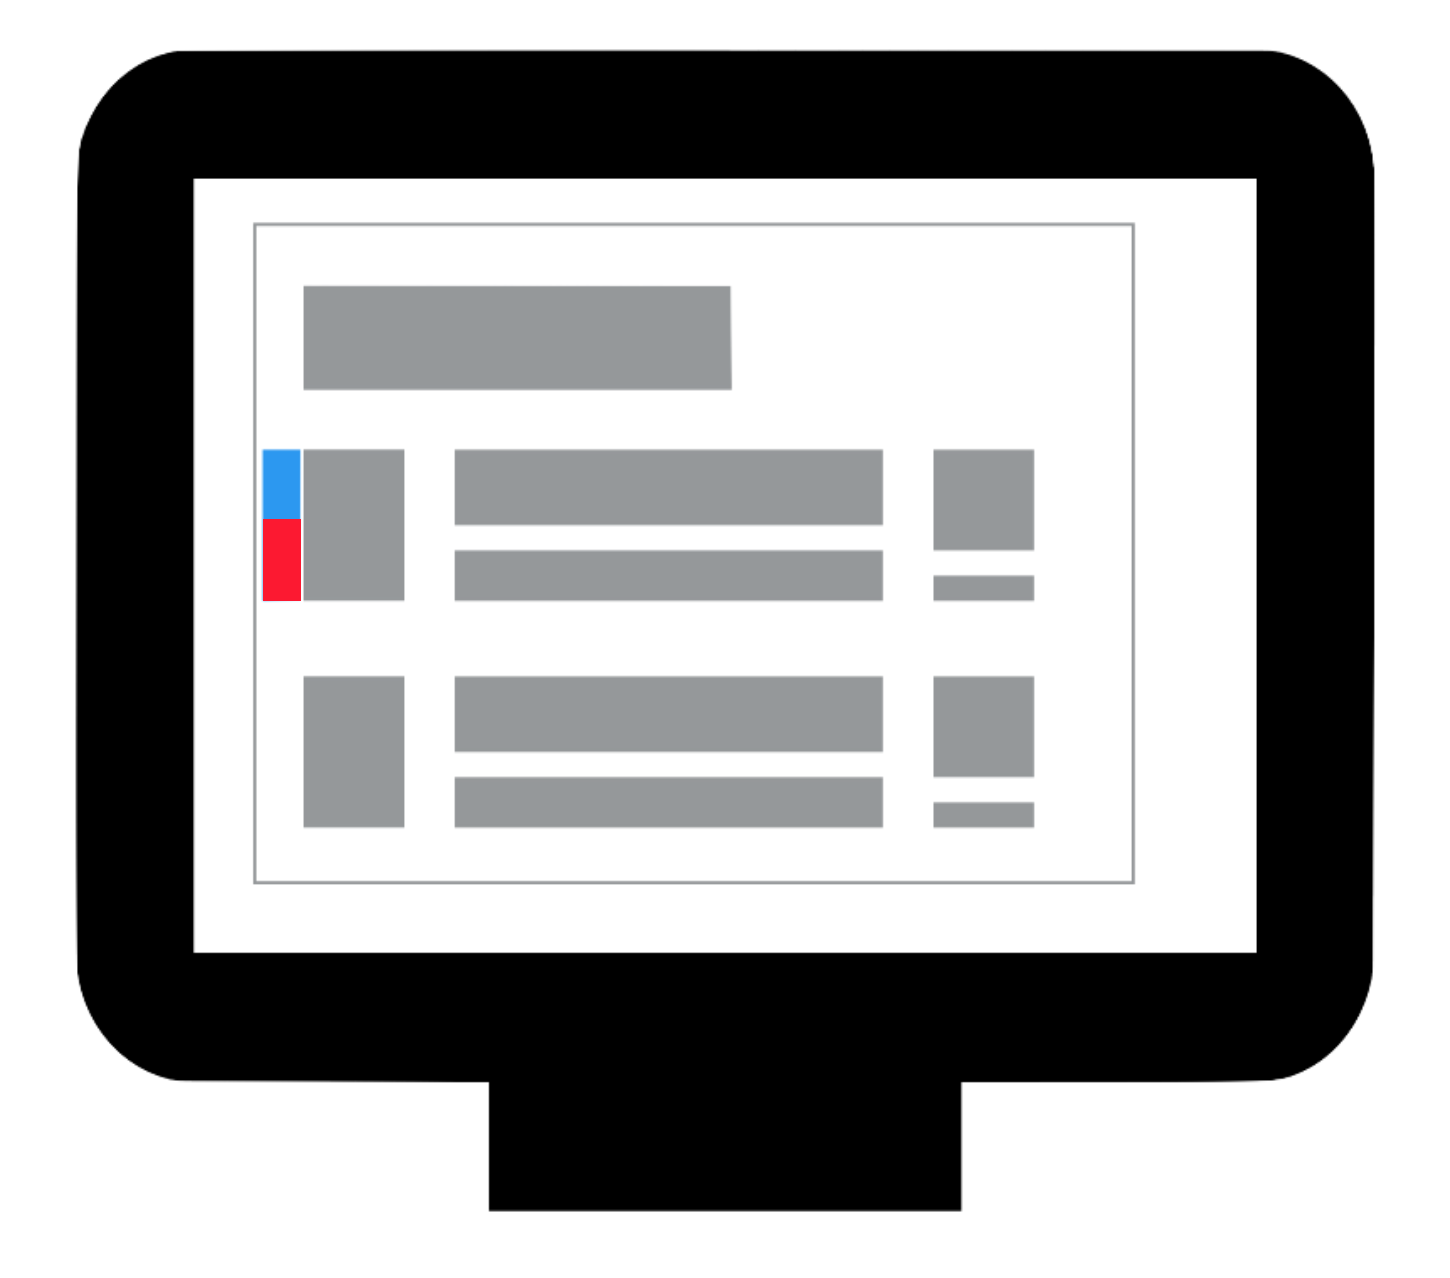
\includegraphics[width=0.4\textwidth]{./images/preference_colour/preference_splited}
  \caption{Preferences on display}

\end{figure}
\newpage
\section{Conclusion}
Displays are a powerful resource to reach a huge audience. Our architecture showed a way to implement custom users personalisation making them even more useful in a closed context such us this University. 

We allows custom based preferences for the Lugano's public transportation giving the advantage to quickly see when a bus is leaving from a previously selected station. Also, an other application, shows the current semester schedules allowing a user to search for other courses.

The preferences are managed using a mobile application served by the MAP Provider to, at the same time, know the global state of each displays and access to all the services availables. Also, is possible to disable the data flow on the fly for certainty applications allowing even more customisation and moving the control power to the user.

In our University, a small environment compared to other well know campus, walk-by contact personalisation really shines and proves is strong utility. Since the displays are deployed into key points such as \emph{Mensa} and \emph{Open Space}, users can easily access to them by just walking.

%%%%%
\newpage
\bibliographystyle{abbrv}
\bibliography{references}
\end{document}